% ****** Start of file apssamp.tex ******
%
%   This file is part of the APS files in the REVTeX 4.1 distribution.
%   Version 4.1r of REVTeX, August 2010
%
%   Copyright (c) 2009, 2010 The American Physical Society.
%
%   See the REVTeX 4 README file for restrictions and more information.
%
% TeX'ing this file requires that you have AMS-LaTeX 2.0 installed
% as well as the rest of the prerequisites for REVTeX 4.1
%
% See the REVTeX 4 README file
% It also requires running BibTeX. The commands are as follows:
%
%  1)  latex apssamp.tex
%  2)  bibtex apssamp
%  3)  latex apssamp.tex
%  4)  latex apssamp.tex
%
\documentclass[
 reprint,
 amsmath,amssymb,
 aps,
 a4paper
]{revtex4-1}

\usepackage[utf8]{inputenc}
\usepackage[spanish]{babel}
\usepackage{hyperref}
\usepackage{datetime}
\usepackage{graphicx}% Include figure files
\usepackage{dcolumn}% Align table columns on decimal point
\usepackage{bm}% bold math
\usepackage{float} % PARA USAR EL [H]
\usepackage{subfig} % PARA PONER SUBFIGURAS
\usepackage{listings} % PARA CODIGO
\usepackage{framed} % PARA CAJITAS
\lstset{ %
  basicstyle=\footnotesize,        % the size of the fonts that are used for the code
  breakatwhitespace=false,         % sets if automatic breaks should only happen at whitespace
  breaklines=true,                 % sets automatic line breaking
  }

\decimalpoint


\begin{document}

\title{Difusión en materia nuclear - Nuclear matter difussion}

\author{Franco Tavella}%
 \email{tavellafran@gmail.com}
\affiliation{%
 Departamento de F\'\i sica, Facultad de Ciencias Exactas y Naturales, Universidad de Buenos Aires,\\
 Pabell\'on I, Ciudad Universitaria, 1428 Buenos Aires, Argentina. 
}%

\author{Lucas Longo}%
 \email{lucaslongo52@gmail.com}
\affiliation{%
 Departamento de F\'\i sica, Facultad de Ciencias Exactas y Naturales, Universidad de Buenos Aires,\\
 Pabell\'on I, Ciudad Universitaria, 1428 Buenos Aires, Argentina. 
}%

\date{\today}

\begin{abstract}
ABSTRACT

\end{abstract}

\maketitle


\section{\label{seq:intro}Introducción}

Potenciales y fuerzas discretizadas que se usan en la simulación, figuras \ref{fig:pots} y \ref{fig:forcs}. Podemos observar comportamientos repulsivos para todos los casos.
\begin{figure}[H]
\centerline{
  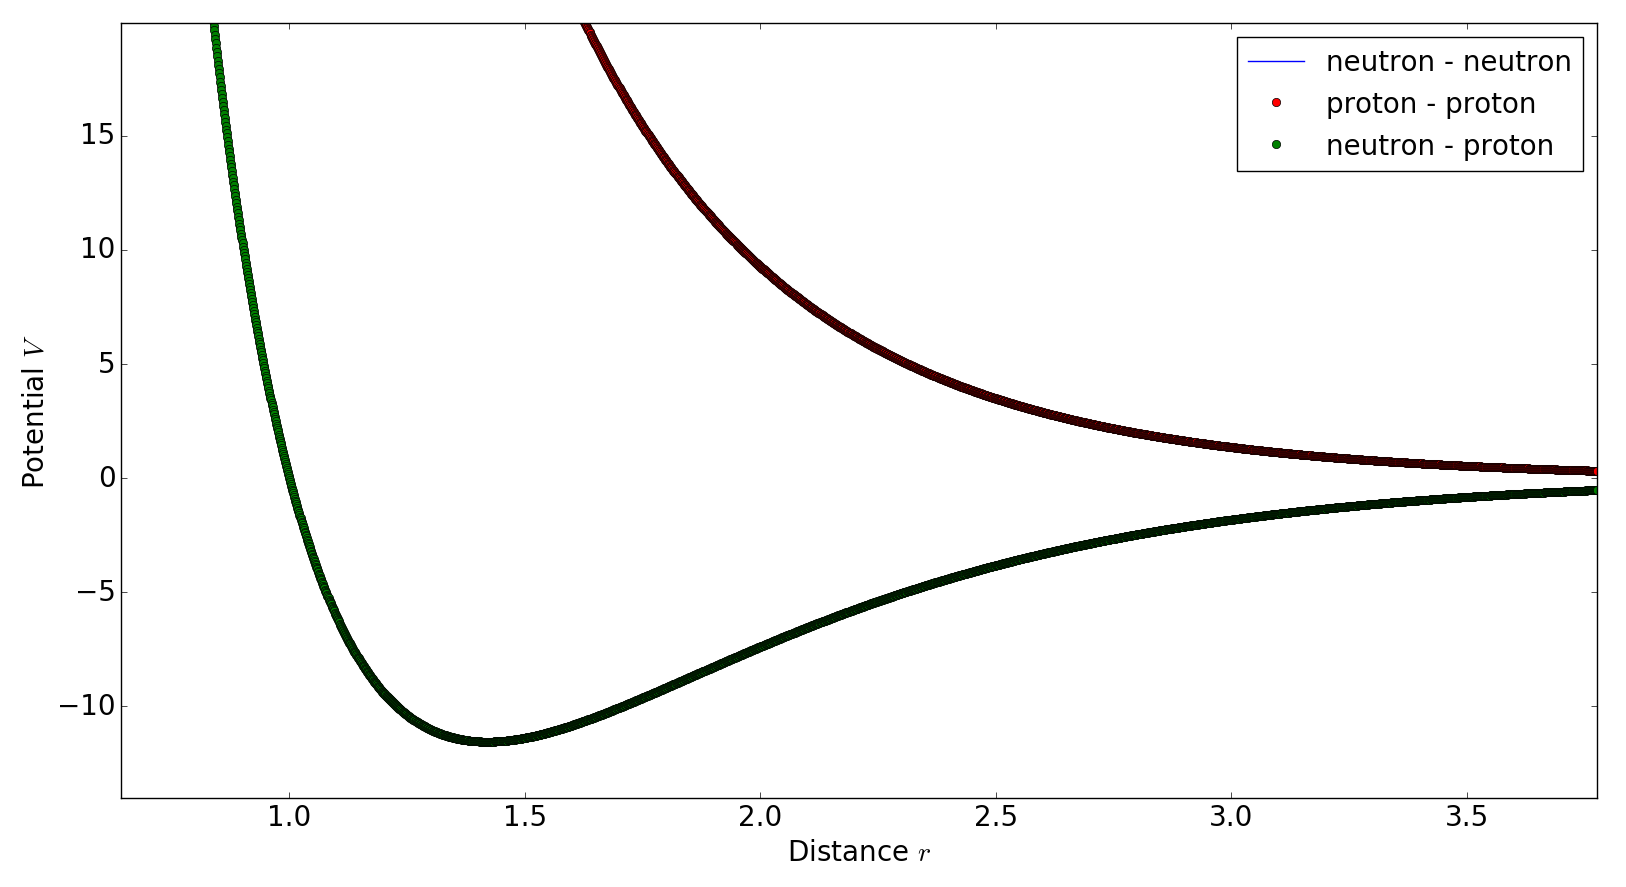
\includegraphics[width=1.0\linewidth]{potentials.png}}
  \caption{\small Potenciales discretizados. Tenemos dos tipos, uno para particulas iguales y otro para particulas diferentes.}
  \label{fig:pots}
\end{figure}

\begin{figure}[H]
\centerline{
  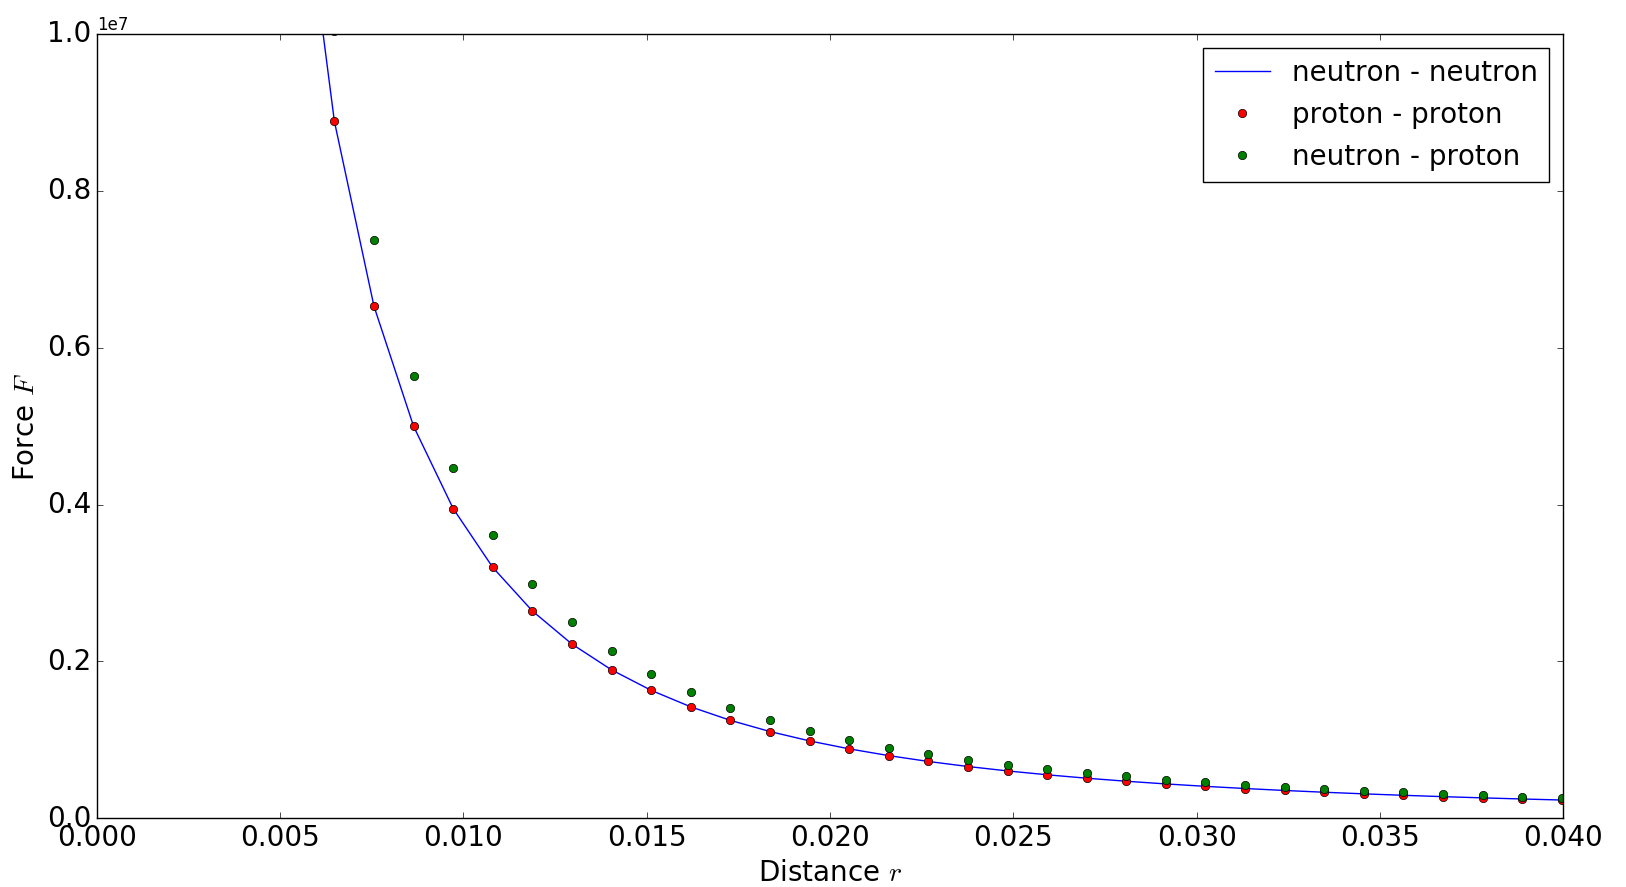
\includegraphics[width=1.0\linewidth]{forces.png}}
  \caption{\small Fuerzas discretizadas. Tenemos dos tipos, uno para particulas iguales y otro para particulas diferentes.}
  \label{fig:forcs}
\end{figure}

\section{\label{seq:difu}Difusión}
La ecuación de difusión describe el comportamiento colectivo de partículas microscópicas que resulta de su movimiento aleatorio. Se puede arribar a ella a partir de la ecuación de continuidad junto con la primer ley fenomenológica de Fick.
\begin{equation}\label{eq:cont}
\frac{\partial \phi}{\partial t} + \nabla \cdot \vec{j}  = 0
\end{equation}
\begin{equation}
\vec{j} = - D(\phi,r)\nabla \phi(r,t)
\end{equation}
en donde $\phi(r,t)$ es la densidad de la sustancia que difunde y $D(\phi,r)$ el coeficiente de difusión colectivo. Para un caso isótropo y homogéneo pensamos a $D(\phi,r) = D$ como una constante y obtenemos una ecuación análoga a la del calor
\begin{equation}\label{eq:difu}
\frac{\partial \phi(r,t)}{\partial t} = D \nabla^{2}\phi(r,t)
\end{equation}

\section{\label{seq:discre}Discretización}
Para la obtención del coeficiente de difusión $D$ debemos resolver la ecuación \ref{eq:difu}. Para ello debemos medir de las simulaciones la cantidad $\phi(r,t)$. Realizaremos una discretización espacial y otra temporal. Utilizaremos los subíndices $i$, $j$ y $k$ para indicar las subceldas espaciales correspondientes a las direcciones $x$, $y$ y $z$ respectivamente. El grillado será isótropo y homogéneo. Temporalmente utilizaremos el subíndice $n$. Entonces tendremos las siguientes cantidades si dividimos cada dirección en $m$ espacios y la caja de simulación posee longitud $L$
\begin{equation}
\phi(r_{i,j,k},t_{n}) = \frac{m^{3}}{L^{3}}N_{i,j,k} 
\end{equation}
en donde $r_{i,j,k}$ representa la posición de la celda i-j-k-ésima y $N_{i,j,k}$ el número de partículas en ésta.
\section{\label{seq:msd}Mean Square Displacement}

La relación de Einstein para difusión establece una relación entre las posiciones de las moléculas y el coeficiente de difusión D.

\begin{equation}\label{eq:rel_einst}
2tD=\frac{1}{3}<[\vec{r}(t)-\vec{r}(t_0)]^2>
\end{equation}

Este resultado es aplicable cuando el tiempo $t$ es largo en comparación al tiempo promedio entre colisiones. Es posible entonces obtener un valor para D:

\begin{equation}\label{eq:D_einst}
D=\lim_{t \to \infty}\frac{<[\vec{r}(t)-\vec{r}(t_0)]^2>}{6t}
\end{equation} 

En las ecuaciones \ref{eq:rel_einst} y \ref{eq:D_einst} el valor $<[\vec{r}(t)-\vec{r}(t_0)]^2>$ es el desplazamiento cuadrático medio $MSD(t)$ del sistema  a tiempo $t$. El símbolo $<>$ debe entenderse como un promedio sobre el número de partículas y sobre orígenes de tiempo $t_0$.

EL coeficiente de difusión $D$ puede también ser evaluado de otras maneras. La relación de Einstein puede reescribirse como:(Ver Haile pág 302)

\begin{equation}\label{eq:D_einst_2}
D=\frac{1}{6}\lim_{t \to \infty}\frac{d}{dt}<[\vec{r}(t)-\vec{r}(t_0)]^2>
\end{equation}

La ecuación \ref{eq:D_einst_2} muestra que $D$ es proporcional a la pendiente del desplazamiento cuadrático medio a tiempos largos. La forma \ref{eq:D_einst_2} se prefiere a la forma \ref{eq:D_einst} en paticular para bajas densidades.\\

El desplazamiento cuadrático medio del sistema de $N$ partículas puede aproximarse como:

\begin{equation}\label{eq:MSD}
MSD(t)=\frac{1}{M.N}\sum_{t_0}^{M}\sum_{i}^{N}[\vec{r}_i(t_0+t)-\vec{r}_i(t_0)]^2
\end{equation}

Donde $N$ es el número de partículas y $M$ es el número de orígenes de tiempo disponibles. Para un total de $L$ pasos temporales separados por $\Delta t$, M depende del tiempo $t$ de la medición mediante: $M=L-\frac{t}{\Delta t}$. 

El algoritmo que hemos utilizado para obtener $MSD(t)$ es el siguiente (ver Haile pág 284):

1) Elegir un valor para el tiempo t

2) Loop sobre orígenes de tiempos $t_j$, $\{j=1,...,M(t)\}$

3) Para cada origen de tiempo $t_o$, loop sobre $i$, $\{i=1,...,N\}$ las $N$ partículas, para leer $\vec{r}_i(t_j+t)$ y $\vec{r}_i(t)$

4) Acumular $[\vec{r}_i(t_{j}+t)-\vec{r}_i(t_{j})]^2$

5) Volver al paso (1) hasta barrer todos los $t$

 nos permite hallar el coeficiente de difusión dado que:

 

\begin{figure}[H]
\centerline{
  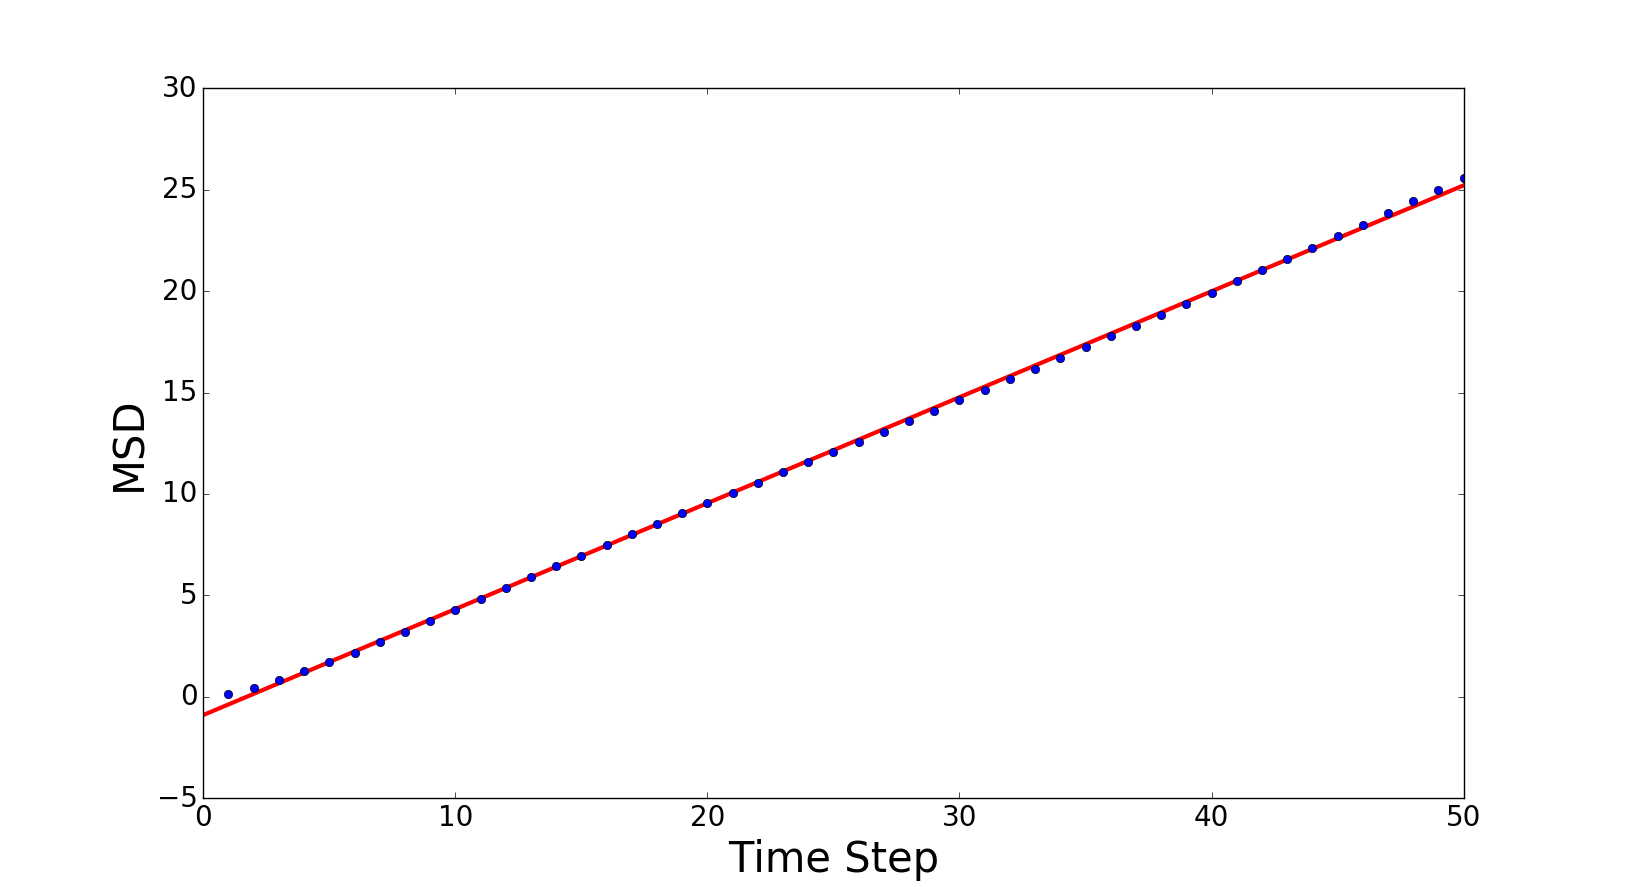
\includegraphics[width=1.0\linewidth]{msdvst.png}}
  \caption{\small MSD para una simulación con posiciones corregidas para eliminar las condiciones periodicas de contorno en función del tiempo. El valor de D obtenido es de $0.087 \pm 0.001$ en unidades de lj.}
  \label{fig:forcs}
\end{figure}

\begin{figure}[H]
\centerline{
  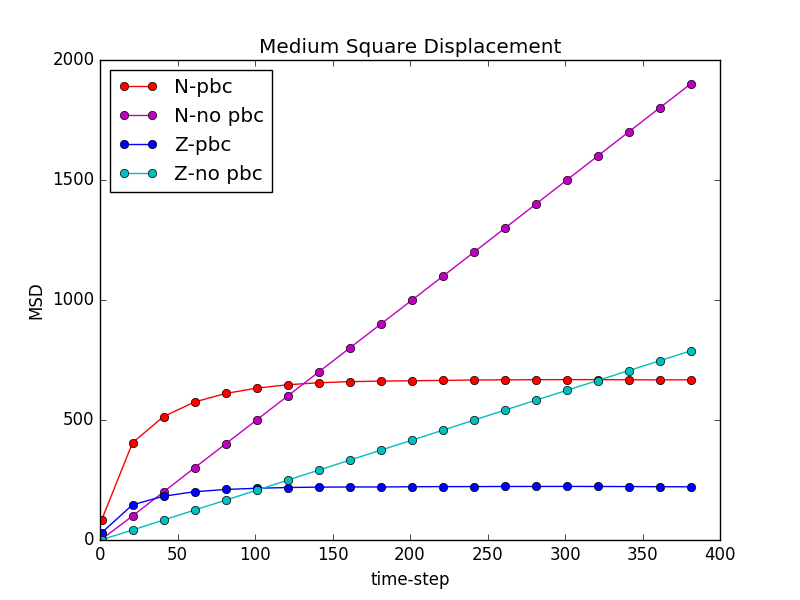
\includegraphics[width=1.0\linewidth]{msd_t400.png}}
  \caption{\small MSD para una simulación con posiciones corregidas para eliminar las condiciones periodicas de contorno en función del tiempo. timestep 0.5 dump 50 run 40000 temp 4.0}
  \label{fig:msd_t400} 
\end{figure}

A partir de la ecuación \ref{eq:D_einst} se calculo $D$ para cada tiempo $t$.

\begin{figure}[H]
\centerline{
  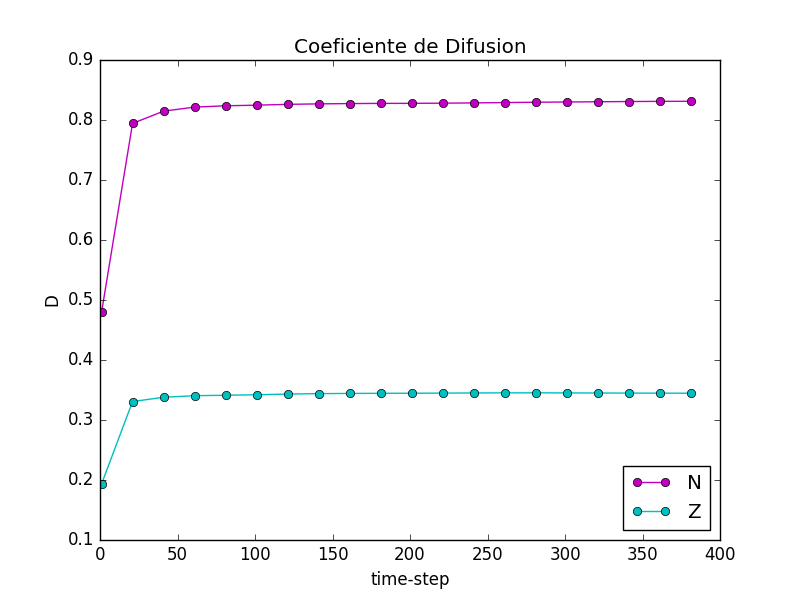
\includegraphics[width=1.0\linewidth]{D_t400.png}}
  \caption{\small Coeficiente de Difusion $D$ para protones($Z$) y neutrones ($N$)}
  \label{fig:D_t400}
\end{figure}

\section{\label{seq:vaf}Velocity Autocorrelation Function}

Las relación de Green-Kubo permite relacionar el desplazamiento cuadrático medio de una cantidad dinámica $A$ con la integral de una funcion de autocorrelación:

 \begin{equation}\label{eq:GK}
 \lim_{t \to \infty} \frac{<[A(t)-A(t_0)]^2>}{2t}=\int_{0}^{\infty}d\tau<\dot{A}(\tau)\dot{A}(\tau_0)>
\end{equation}

En particular para el coeficiente de difusión, la relación de Green-Kubo es:

 \begin{equation}\label{eq:GK_D}
 D=\frac{1}{3}\int_{0}^{\infty}dt<\vec{v}(t)\vec{v}(t_0)>
\end{equation}

Aquí $<\vec{v}(t)\vec{v}(t_0)>$ es la función de autocorrelación de velocidades $VACF(t)$. Nuevamente el símbolo $<>$ indica un promedio sobre el número de partículas y sobre orígenes de tiempos $t_0$.

Para calcular $VACF(t)$ hemos utilizado nuevamente el algoritmo ya usado para el $MSD(t)$:

\begin{equation}\label{eq:MSD}
VACF(t)=\frac{1}{M.N}\sum_{t_0}^{M}\sum_{i}^{N}\vec{v}_i(t_0).\vec{v}_i(t_0+t)
\end{equation}

\begin{figure}[H]
\centerline{
  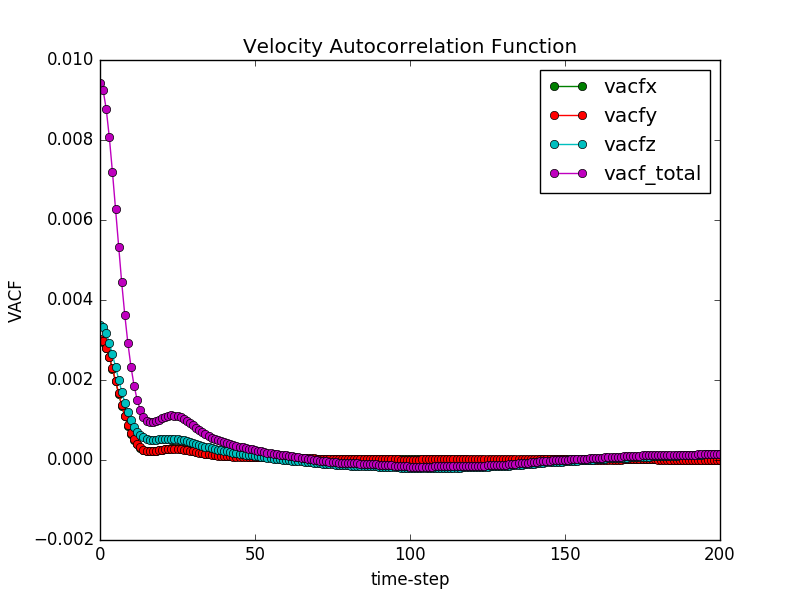
\includegraphics[width=1.0\linewidth]{vacf_N_200.png}}
  \caption{\small Función de autocorrelación de velocidades para neutrones. timestep 0.02 dump 50 run 20000 temp 4.0}
  \label{fig:vacf_N_200}
\end{figure}

\begin{figure}[H]
\centerline{
  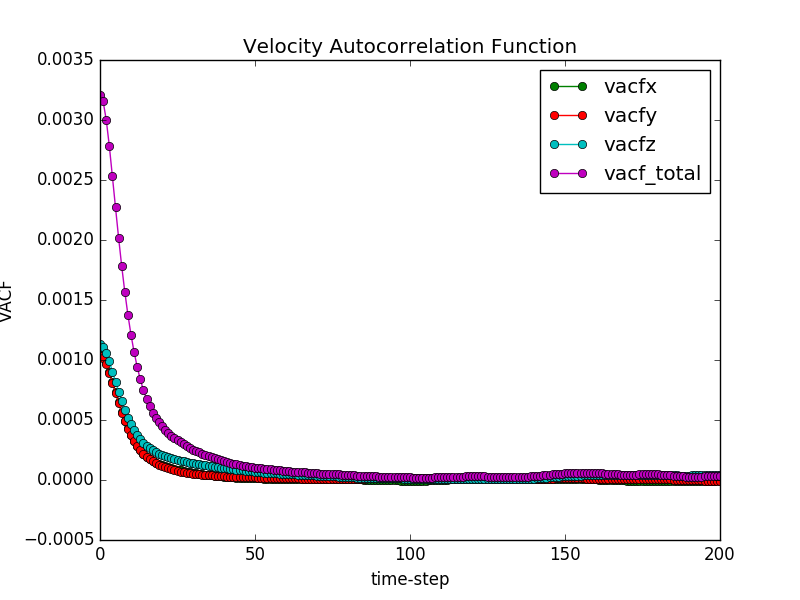
\includegraphics[width=1.0\linewidth]{vacf_Z_200.png}}
  \caption{\small Función de autocorrelación de velocidades para protones. timestep 0.02 dump 50 run 20000 temp 4.0}
  \label{fig:vacf_Z_200}
\end{figure}

\begin{figure}
\centerline{
  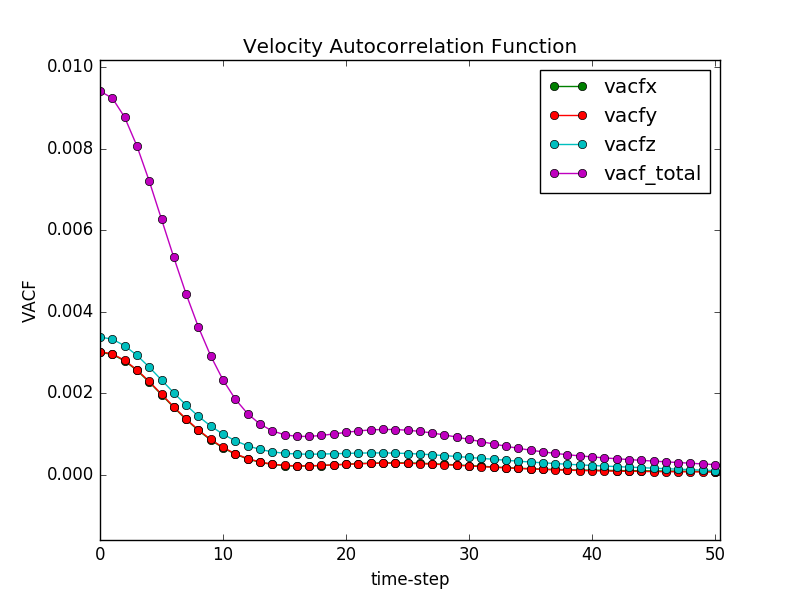
\includegraphics[width=1.0\linewidth]{vacf_N_50.png}}
  \caption{\small Función de autocorrelación de velocidades para neutrones. (Zoom)}
  \label{fig:vacf_N_50}
\end{figure}

\begin{figure}
\centerline{
  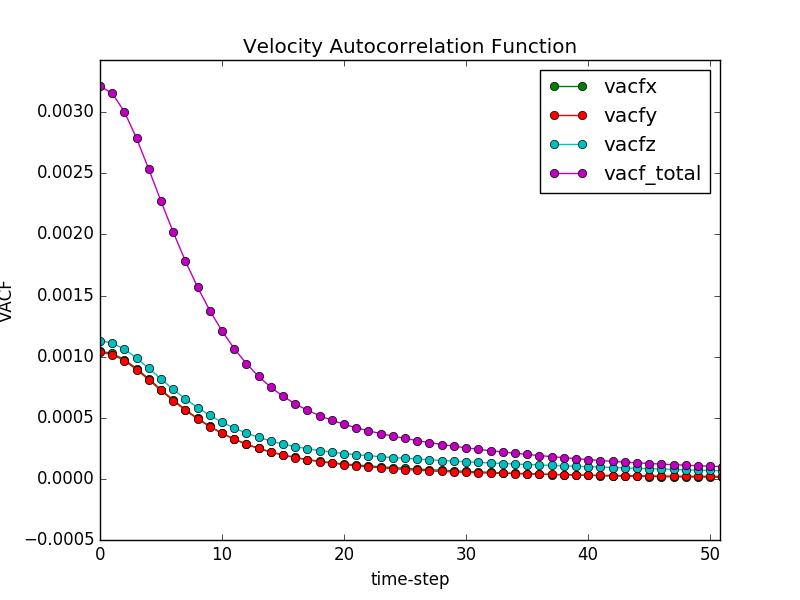
\includegraphics[width=1.0\linewidth]{vacf_Z_50.png}}
  \caption{\small Función de autocorrelación de velocidades para protones. (Zoom)}
  \label{fig:vacf_Z_50}
\end{figure}

\section{\label{seq:details}Detalles técnicos}
Las posiciones de las partículas son obtenidas a través del comando $dump$ en LAMMPS. En la documentación\cite{dumplammps} sobre este comando se hace una aclaración sobre las condiciones periódicas de contorno
\begin{framed}
\textit{Because periodic boundary conditions are enforced only on timesteps when neighbor lists are rebuilt, the coordinates of an atom written to a dump file may be slightly outside the simulation box. Re-neighbor timesteps will not typically coincide with the timesteps dump snapshots are written. See the dump\_ modify pbc command if you with to force coordinates to be strictly inside the simulation box.}
\end{framed}


\begin{thebibliography}{9}

\bibitem{dumplammps}
  Sandia National Laboratories,
  \url{http://lammps.sandia.gov/doc/dump.html},
  Consultado 02/09/17

\end{thebibliography}

\end{document}

